\documentclass[10pt,aspectratio=169]{beamer}
\usepackage[T1]{fontenc}
\usepackage{booktabs}
\usepackage{xcolor}
\usepackage{tikz}
\usetikzlibrary{arrows,shapes,positioning,fit,backgrounds}
\usetheme{metropolis}

% Color definitions
\definecolor{darkblue}{RGB}{23, 73, 137}
\definecolor{accent}{RGB}{0, 163, 224}
\definecolor{lightblue}{RGB}{230, 242, 255}
\definecolor{lightgreen}{RGB}{240, 255, 240}
\definecolor{lightyellow}{RGB}{255, 255, 224}

\title{Health Informatics and Universal Health Coverage (UHC)}
\subtitle{SDS6210 – Informatics for Health \\ MSc Public Health Data Science}
\author{Cavin Otieno}
\institute{Department of Public Health}
\date{\today}

\begin{document}

%=======================================================================
% TITLE FRAME
%=======================================================================
{
\setbeamertemplate{footline}{}
\begin{frame}
    \titlepage
\end{frame}
}

%=======================================================================
% OUTLINE
%=======================================================================
\section{Outline}
\begin{frame}{Presentation Outline}
    \begin{enumerate}
        \item Universal Health Coverage: Definitions and Dimensions
        \item WHO Health System Building Blocks Framework
        \item Health Informatics Tools and Technologies
        \item Mapping Informatics Contributions to UHC
        \item Real-World Applications in LMICs
        \item Critical Analysis: Limitations and Challenges
        \item Efficiency, Accountability, and Population Health Outcomes
        \item Policy and Public Health Implications
        \item Conclusions
    \end{enumerate}
\end{frame}

%=======================================================================
% SECTION 1: UNIVERSAL HEALTH COVERAGE
%=======================================================================
\section{Universal Health Coverage: Definitions and Dimensions}

\begin{frame}{What is Universal Health Coverage?}
    \begin{block}{WHO Definition}
        Universal Health Coverage (UHC) means that ``all people have access to the full spectrum of quality health services they need, when and where they need them, without financial hardship'' \cite{who2019}. It encompasses the full continuum of essential health services, from health promotion to prevention, treatment, rehabilitation, and palliative care.
    \end{block}
    
    \pause
    
    \begin{itemize}
        \item \textbf{Population Coverage}: Who is covered? Ensuring all population groups, including marginalized and hard-to-reach populations, have access to services
        \item \textbf{Service Coverage}: What services are covered? Providing a comprehensive package of essential health interventions across the care continuum
        \item \textbf{Financial Protection}: How much does it cost? Ensuring that health payments do not push people into poverty or cause catastrophic expenditure
    \end{itemize}
\end{frame}

\begin{frame}{UHC Dimensions: Service Coverage}
    \begin{center}
        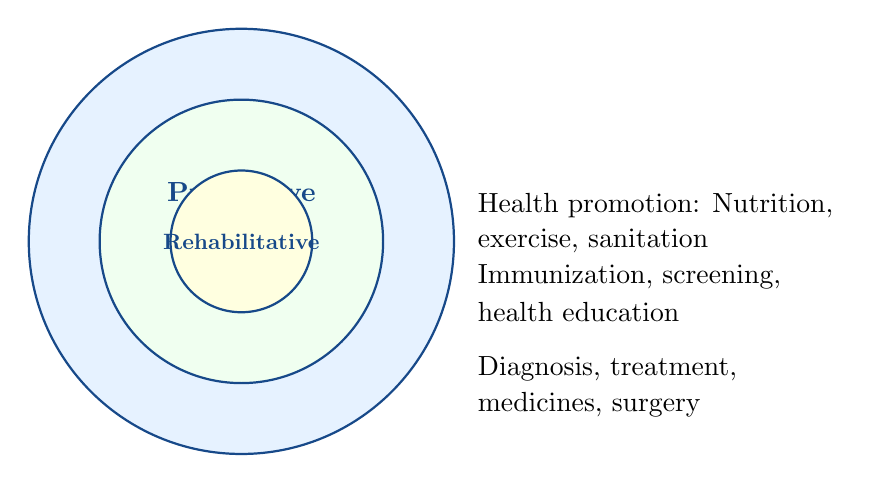
\begin{tikzpicture}[scale=0.9]
            % Three concentric circles
            \draw[fill=lightblue, draw=darkblue, thick] (0,0) circle (3cm);
            \node[darkblue, font=\bfseries] at (0,0) {Promotive};
            
            \draw[fill=lightgreen, draw=darkblue, thick] (0,0) circle (2cm);
            \node[darkblue, font=\bfseries] at (0,0.7) {Preventive};
            \node[darkblue, font=\bfseries] at (0,-0.3) {Curative};
            
            \draw[fill=lightyellow, draw=darkblue, thick] (0,0) circle (1cm);
            \node[darkblue, font=\bfseries, scale=0.8] at (0,0) {Rehabilitative};
            
            % Labels outside
            \node[anchor=west] at (3.2,0.5) {Health promotion: Nutrition,};
            \node[anchor=west] at (3.2,0) {exercise, sanitation};
            \node[anchor=west] at (3.2,-0.5) {Immunization, screening,};
            \node[anchor=west] at (3.2,-1) {health education};
            \node[anchor=west] at (3.2,-1.8) {Diagnosis, treatment,};
            \node[anchor=west] at (3.2,-2.3) {medicines, surgery};
        \end{tikzpicture}
    \end{center}
    
    \smallskip
    
    Service coverage includes promotive, preventive, curative, rehabilitative, and palliative care services across the lifespan. The Lancet UHC Global Monitoring Database tracks coverage of essential health service interventions across 204 countries \cite{fullman2018}.
\end{frame}

\begin{frame}{UHC Dimensions: Financial Risk Protection}
    \begin{columns}
        \begin{column}{0.5\textwidth}
            \begin{block}{Financial Protection Indicators}
                \begin{itemize}
                    \item \textbf{Incidence of catastrophic health spending}: Households spending more than 10\% or 25\% of total household consumption or income on out-of-pocket health expenses
                    \item \textbf{Impoverishment due to health spending}: Households pushed below the poverty line by health expenditures
                    \item \textbf{Service utilization without financial ruin}: Ability to access care without selling assets or borrowing
                \end{itemize}
            \end{block}
        \end{column}
        \begin{column}{0.5\textwidth}
            \begin{block}{The Poverty Connection}
                An estimated 100 million people are pushed into extreme poverty annually due to out-of-pocket health expenses, while 800 million spend at least 10\% of their household budgets on healthcare \cite{who2019}. This financial toxicity directly undermines UHC objectives.
            \end{block}
        \end{column}
    \end{columns}
    
    \pause
    
    \begin{block}{UHC Target 3.8}
        Target 3.8 of the Sustainable Development Goals specifically calls for achieving financial risk protection, noting that without addressing affordability, access alone is insufficient to achieve UHC.
    \end{block}
\end{frame}

\begin{frame}{UHC Dimensions: Equity and Access}
    \begin{center}
        \begin{tabular}{@{}lp{6cm}@{}}
            \toprule
            \textbf{Dimension} & \textbf{Description} \\
            \midrule
            \textbf{Geographic Access} & Physical availability of health facilities and workforce, particularly in rural and remote areas \\
            \textbf{Economic Access} & Affordability of services, including direct costs and indirect costs (transport, lost wages) \\
            \textbf{Socio-cultural Access} & Acceptability of services, language accessibility, cultural appropriateness \\
            \textbf{Information Access} & Awareness of available services and health literacy to navigate health systems \\
            \textbf{Quality Access} & Services must be effective, safe, and responsive to user expectations \\
            \bottomrule
        \end{tabular}
    \end{center}
    
    \pause
    
    \begin{block}{The Equity Imperative}
        UHC is fundamentally an equity concept. A health system that provides excellent care to urban populations while excluding rural communities, the poor, or marginalized groups has not achieved universal coverage. Equity-focused monitoring disaggregates coverage by wealth quintile, geography, sex, and other stratifiers \cite{boerma2014}.
    \end{block}
\end{frame}

%=======================================================================
% SECTION 2: WHO HEALTH SYSTEM BUILDING BLOCKS
%=======================================================================
\section{WHO Health System Building Blocks Framework}

\begin{frame}{The WHO Framework}
    \begin{center}
        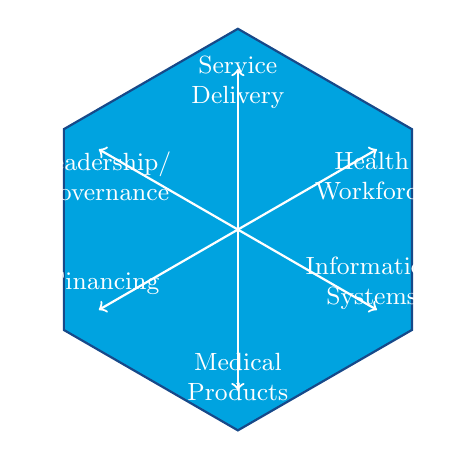
\begin{tikzpicture}[scale=0.85]
            % Central hexagon
            \draw[fill=darkblue, draw=none] (0,0) circle (1.5cm);
            \node[white, font=\bfseries, align=center] at (0,0) {Health\\Outcomes};
            
            % Outer hexagons
            \draw[fill=accent, draw=darkblue, thick] (0,3) -- (2.6,1.5) -- (2.6,-1.5) -- (0,-3) -- (-2.6,-1.5) -- (-2.6,1.5) -- cycle;
            
            % Block labels
            \node[white, font=\small, align=center] at (0,2.2) {Service\\Delivery};
            \node[white, font=\small, align=center] at (2,0.8) {Health\\Workforce};
            \node[white, font=\small, align=center] at (2,-0.8) {Information\\Systems};
            \node[white, font=\small, align=center] at (0,-2.2) {Medical\\Products};
            \node[white, font=\small, align=center] at (-2,-0.8) {Financing};
            \node[white, font=\small, align=center] at (-2,0.8) {Leadership/\\Governance};
            
            % Arrows
            \foreach \a in {30, 90, 150, 210, 270, 330} {
                \draw[->, thick, white] (0,0) -- (\a:2.4);
            }
        \end{tikzpicture}
    \end{center}
    
    \smallskip
    
    The WHO health systems framework identifies six building blocks that must function together to achieve health system goals. Health information systems (HIS) serve as the ``backbone'' that supports decision-making across all other blocks \cite{who2007}.
\end{frame}

\begin{frame}{Health Information Systems as the Backbone}
    \begin{columns}
        \begin{column}{0.55\textwidth}
            \begin{block}{HIS Contributions to Each Block}
                \begin{itemize}
                    \item \textbf{Service Delivery}: Facility-level data on utilization, quality, and efficiency
                    \item \textbf{Health Workforce}: Tracking workforce distribution, training, and performance
                    \item \textbf{Medical Products}: Supply chain monitoring, stock levels, rational use
                    \item \textbf{Financing}: Claims processing, expenditure tracking, resource allocation
                    \item \textbf{Leadership}: Evidence for policy, monitoring of commitments
                \end{itemize}
            \end{block}
        \end{column}
        \begin{column}{0.45\textwidth}
            \begin{block}{The Feedback Loop}
                High-functioning HIS generate data that informs decisions across all blocks, while well-functioning blocks generate the data needed for HIS. Weakness in any component creates ripple effects throughout the system.
            \end{block}
        \end{column}
    \end{columns}
    
    \pause
    
    \begin{block}{System Strengthening Perspective}
        Investments in health informatics must be understood as system-wide interventions, not isolated technology projects. TheHIS should be conceptualized as the nervous system of the health sector.
    \end{block}
\end{frame}

%=======================================================================
% SECTION 3: HEALTH INFORMATICS TOOLS AND TECHNOLOGIES
%=======================================================================
\section{Health Informatics Tools and Technologies}

\begin{frame}{Health Informatics Landscape}
    \begin{center}
        \begin{tikzpicture}[scale=0.8]
            % Four quadrants
            \draw[fill=lightblue, draw=darkblue, thick] (0,0) rectangle (6,4);
            \node[darkblue, font=\bfseries] at (3,3.5) {Clinical Informatics};
            \node[anchor=center] at (3,2) {EHRs, Clinical Decision\\Support, CPOE};
            \node[anchor=center] at (3,0.7) {Telemedicine, ePrescribing};
            
            \draw[fill=lightgreen, draw=darkblue, thick] (6,0) rectangle (12,4);
            \node[darkblue, font=\bfseries] at (9,3.5) {Public Health Informatics};
            \node[anchor=center] at (9,2) {Surveillance, Reporting,\\Contact Tracing};
            \node[anchor=center] at (9,0.7) {Outbreak Investigation, GIS};
            
            \draw[fill=lightyellow, draw=darkblue, thick] (0,-4) rectangle (6,0);
            \node[darkblue, font=\bfseries] at (3,-3.5) {Consumer Health Informatics};
            \node[anchor=center] at (3,-2) {mHealth\\Apps, Wearables};
            \node[anchor=center] at (3,-3.3) {Patient-Reported Outcomes};
            
            \draw[fill=lightpink, draw=darkblue, thick] (6,-4) rectangle (12,0);
            \node[darkblue, font=\bfseries] at (9,-3.5) {Health Administration Informatics};
            \node[anchor=center] at (9,-2) {Claims Processing,\\Registry Management};
            \node[anchor=center] at (9,-3.3) {Supply Chain, HR Systems};
        \end{tikzpicture}
    \end{center}
    
    \smallskip
    
    Health informatics encompasses multiple domains that collectively support health system functions. For UHC, the integration of these domains is essential for comprehensive system strengthening \cite{yasnoff2009}.
\end{frame}

%=======================================================================
% SECTION 4: EHRs AND UHC
%=======================================================================
\section{Electronic Health Records and UHC}

\begin{frame}{EHRs Enabling UHC: Service Coverage}
    \begin{columns}
        \begin{column}{0.5\textwidth}
            \begin{block}{Clinical Decision Support}
                \begin{itemize}
                    \item Evidence-based treatment protocols integrated into workflow
                    \item Drug-drug and drug-allergy interaction checking
                    \item Clinical reminders for preventive services (immunization, screening)
                    \item Risk stratification algorithms for chronic disease management
                \end{itemize}
            \end{block}
        \end{column}
        \begin{column}{0.5\textwidth}
            \begin{block}{Continuity of Care}
                \begin{itemize}
                    \item Longitudinal patient records across providers and facilities
                    \item Referral management with structured information exchange
                    \item Care coordination for complex patients
                    \item Reduced duplication of tests and procedures
                \end{itemize}
            \end{block}
        \end{column}
    \end{columns}
    
    \pause
    
    \begin{block}{Ethiopia Example}
        The Ethiopian Health Extension Program implemented the Family Folder System, an EHR adapted for primary care, which supported the expansion of essential health services to 85\% of the population through improved tracking of preventive interventions and continuity of care for chronic conditions \cite{braa2012}.
    \end{block}
\end{frame}

\begin{frame}{EHRs Enabling UHC: Financial Protection}
    \begin{center}
        \begin{tabular}{@{}lp{6cm}@{}}
            \toprule
            \textbf{Mechanism} & \textbf{Contribution to Financial Protection} \\
            \midrule
            Claims processing automation & Reduced administrative costs, faster reimbursement \\
            Fraud detection & Prevents leakage of funds to fraudulent providers \\
            Utilization review & Identifies unnecessary procedures, reduces waste \\
            Essential medicines tracking & Ensures availability, reduces informal payments \\
            Capitation management & Enables provider payment reform based on registered populations \\
            \bottomrule
        \end{tabular}
    \end{center}
    
    \pause
    
    \begin{block}{Thailand's Experience}
        Thailand's Universal Coverage Scheme, covering 47 million citizens, relies heavily on its NHSO information system for claims processing, fraud detection, and quality monitoring. The system processes over 500 million claims annually while keeping administrative costs below 5\% of total health expenditure \cite{sakthong2016}.
    \end{block}
\end{frame}

\begin{frame}{EHRs Enabling UHC: Equity}
    \begin{itemize}
        \item \textbf{Population Registries}: EHRs maintain population registries that enable outreach to underserved groups and tracking of coverage gaps
        \item \textbf{Disaggregation Capabilities}: Data can be stratified by socioeconomic status, geography, and other equity dimensions to identify disparities
        \item \textbf{Outreach Automation}: Reminder systems can target populations lagging in preventive service uptake
        \item \textbf{Community Health Worker Integration}: EHRs linked to community health information systems extend reach to marginalized populations
    \end{itemize}
    
    \pause
    
    \begin{block}{Brazil's Family Health Strategy}
        Brazil's Estratégia Saúde da Família (ESF) uses the Sistema de Informação da Atenção Básica (SIAB) to monitor primary care coverage and equity. The system enables identification of underserved micro-areas and guides deployment of community health agents to reduce geographic inequities in access \cite{macinko2014}.
    \end{block}
\end{frame}

%=======================================================================
% SECTION 5: HEALTH INFORMATION SYSTEMS (DHIS2)
%=======================================================================
\section{Health Information Systems and DHIS2}

\begin{frame}{DHIS2: A Global Public Health Good}
    \begin{columns}
        \begin{column}{0.5\textwidth}
            \begin{block}{DHIS2 Overview}
                \begin{itemize}
                    \item Open-source health information platform developed by the University of Oslo
                    \item Used in over 70 countries, serving 2 billion people
                    \item Supports aggregate data collection, event tracking, and individual-level data
                    \item Designed for low-resource settings with offline capabilities
                    \item Flexible data model adaptable to local contexts
                \end{itemize}
            \end{block}
        \end{column}
        \begin{column}{0.5\textwidth}
            \begin{block}{Core Functions}
                \begin{itemize}
                    \item Data capture at facility, district, and national levels
                    \item Automated validation and data quality checks
                    \item Dashboard visualization for data-driven decision-making
                    \item Integration with health facility registries
                    \item Support for disease surveillance and outbreak response
                \end{itemize}
            \end{block}
        \end{column}
    \end{columns}
    
    \pause
    
    \begin{block}{Open Source Philosophy}
        DHIS2's open-source model makes it a ``global public good,'' enabling countries to own and customize their health information systems without vendor lock-in while contributing to a global community of practice \cite{braa2012}.
    \end{block}
\end{frame}

\begin{frame}{DHIS2 Supporting UHC Monitoring}
    \begin{center}
        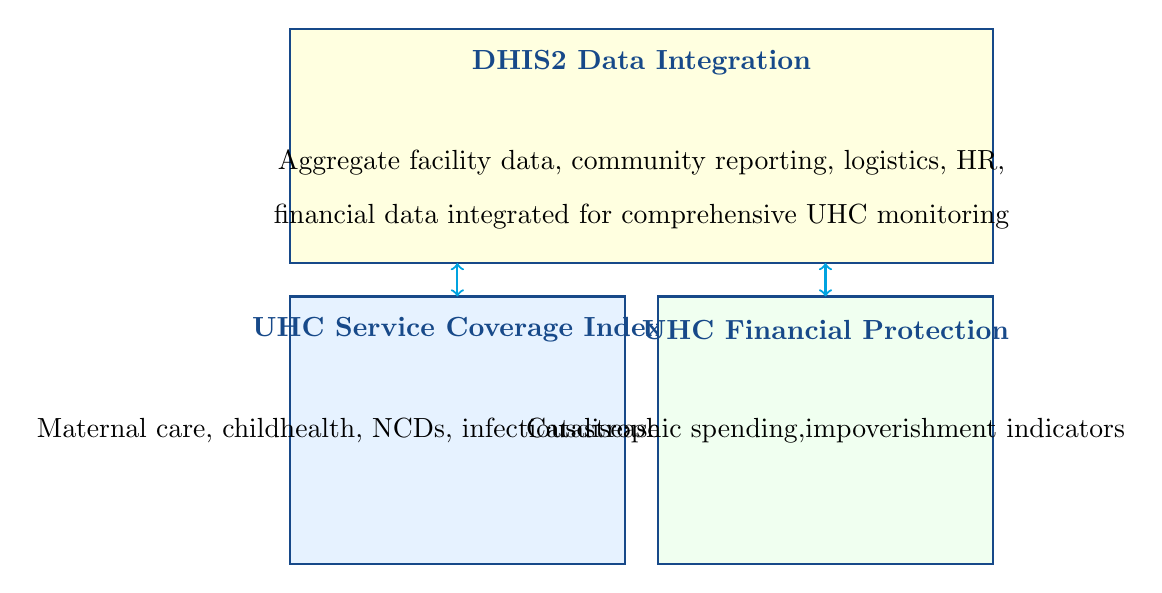
\begin{tikzpicture}[scale=0.85]
            % UHC cube
            \draw[fill=lightblue, draw=darkblue, thick] (0,0) rectangle (5,4);
            \node[darkblue, font=\bfseries] at (2.5,3.5) {UHC Service Coverage Index};
            \node[anchor=center] at (2.5,2) {Maternal care, child\\health, NCDs, infectious\\diseases, service capacity};
            
            \draw[fill=lightgreen, draw=darkblue, thick] (5.5,0) rectangle (10.5,4);
            \node[darkblue, font=\bfseries] at (8,3.5) {UHC Financial Protection};
            \node[anchor=center] at (8,2) {Catastrophic spending,\\impoverishment indicators};
            
            \draw[fill=lightyellow, draw=darkblue, thick] (0,4.5) rectangle (10.5,8);
            \node[darkblue, font=\bfseries] at (5.25,7.5) {DHIS2 Data Integration};
            \node[anchor=center] at (5.25,6) {Aggregate facility data, community reporting, logistics, HR,};
            \node[anchor=center] at (5.25,5.2) {financial data integrated for comprehensive UHC monitoring};
            
            % Connecting arrows
            \draw[<->, thick, accent] (2.5,4) -- (2.5,4.5);
            \draw[<->, thick, accent] (8,4) -- (8,4.5);
        \end{tikzpicture}
    \end{center}
    
    \smallskip
    
    DHIS2 supports the calculation of UHC service coverage indices by integrating data across multiple program areas, enabling countries to track progress toward SDG 3.8 and identify service coverage gaps \cite{nicholls2021}.
\end{frame}

\begin{frame}{DHIS2 Case Study: Ghana}
    \begin{columns}
        \begin{column}{0.5\textwidth}
            \begin{block}{Implementation}
                \begin{itemize}
                    \item National deployment since 2012
                    \item Over 6,000 health facilities reporting
                    \item Integrated disease surveillance and response
                    \item Maternal health monitoring
                    \item Health worker task tracking
                \end{itemize}
            \end{block}
        \end{column}
        \begin{column}{0.5\textwidth}
            \begin{block}{UHC Outcomes}
                \begin{itemize}
                    \item Antenatal care coverage increased from 79\% to 97\%
                    \item Skilled birth attendance improved from 55\% to 79\%
                    \item Facility-based deliveries rose from 54\% to 74\%
                    \item Data quality scores improved from 40\% to 85\%
                    \item Real-time surveillance enabled rapid outbreak response
                \end{itemize}
            \end{block}
        \end{column}
    \end{columns}
    
    \pause
    
    \begin{block}{Key Success Factors}
        Ghana's DHIS2 success is attributed to government ownership, integration with existing systems, capacity building at all levels, and use of data for decision-making at district and facility levels \cite{odhiambo2019}.
    \end{block}
\end{frame}

%=======================================================================
% SECTION 6: mHEALTH AND TELEMEDICINE
%=======================================================================
\section{mHealth and Telemedicine}

\begin{frame}{mHealth for Service Coverage}
    \begin{columns}
        \begin{column}{0.5\textwidth}
            \begin{block}{Access Extension}
                \begin{itemize}
                    \item Mobile phone penetration exceeds 80\% in most LMICs
                    \item Reaches populations beyond physical facility reach
                    \item Supports community health worker programs
                    \item Enables appointment reminders and health promotion
                    \item Facilitates remote symptom screening and triage
                \end{itemize}
            \end{block}
        \end{column}
        \begin{column}{0.5\textwidth}
            \begin{block}{Service Delivery Innovation}
                \begin{itemize}
                    \item SMS-based appointment reminders (no-show reduction of 30-50\%)
                    \item Interactive voice response for health information
                    \item Mobile-based contact tracing (essential for outbreak response)
                    \item Photo-based diagnostic support (dermatology, ophthalmology)
                    \item Medication adherence support through reminders
                \end{itemize}
            \end{block}
        \end{column}
    \end{columns}
    
    \pause
    
    \begin{block}{The mHealth Evidence Gap}
        While mHealth pilot projects show promise, systematic reviews find weak evidence for sustained health impact. The WHO Global Observatory for eHealth notes that only 7\% of mHealth initiatives have been rigorously evaluated \cite{who2019}.
    \end{block}
\end{frame}

\begin{frame}{Telemedicine for Equity}
    \begin{center}
        \begin{tabular}{@{}lp{6cm}@{}}
            \toprule
            \textbf{Model} & \textbf{Contribution to UHC Equity} \\
            \midrule
            Store-and-forward telemedicine & Specialist consultations without patient travel; asynchronous review of cases \\
            Real-time video consultation & Direct specialist access for rural patients; virtual rounds \\
            Hub-and-spoke networks & District hospitals connected to tertiary centers for support \\
            Telementoring (e.g., Project ECHO) & Capacity building of primary providers through virtual communities of practice \\
            Remote patient monitoring & Chronic disease management without frequent facility visits \\
            \bottomrule
        \end{tabular}
    \end{center}
    
    \pause
    
    \begin{block}{India's eSanjeevani}
        India's national telemedicine platform, eSanjeevani, has conducted over 14 million consultations since 2020, providing specialist access to rural populations that would otherwise require travel to urban centers. The platform is being integrated with Ayushman Bharat health insurance to create a seamless care pathway \cite{mohfw2021}.
    \end{block}
\end{frame}

\begin{frame}{mHealth for Financial Protection}
    \begin{itemize}
        \item \textbf{Mobile Money Integration}: Mobile-based insurance premium collection and claims payment reduce administrative costs and expand financial access to rural populations
        \item \textbf{Voucher Systems}: Mobile-based conditional cash transfers and health service vouchers improve targeting and reduce leakage
        \item \textbf{Transport Subsidies}: Mobile systems can coordinate and reimburse transport costs for patients requiring referral
        \item \textbf{Pre-authorization Systems}: Mobile pre-authorization for planned procedures reduces surprise billing and enables planning
    \end{itemize}
    
    \pause
    
    \begin{block}{Kenya's M-TIBA}
        M-TIBA, a mobile health wallet platform in Kenya, enables individuals to save, receive, and pay for health services using mobile money. Linked to Kenya's national health insurance, it has enrolled over 4 million users and demonstrably increased utilization of preventive services among low-income populations \cite{gelb2019}.
    \end{block}
\end{frame}

%=======================================================================
% SECTION 7: DIGITAL HEALTH FINANCING AND REGISTRIES
%=======================================================================
\section{Digital Health Financing and Registries}

\begin{frame}{Digital Financial Systems for UHC}
    \begin{columns}
        \begin{column}{0.5\textwidth}
            \begin{block}{Insurance Administration}
                \begin{itemize}
                    \item Population registries linked to eligibility databases
                    \item Automated premium collection and subsidy management
                    \item Real-time claims processing with fraud detection
                    \item Capitation management and performance-based payment
                    \item Portable benefits across providers and regions
                \end{itemize}
            \end{block}
        \end{column}
        \begin{column}{0.5\textwidth}
            \begin{block}{Resource Allocation}
                \begin{itemize}
                    \item Needs-based resource distribution formulas
                    \item Utilization tracking to identify under-served areas
                    \item Performance monitoring for accountability
                    \item Expenditure tracking for financial sustainability
                    \item Evidence for budget advocacy and allocation
                \end{itemize}
            \end{block}
        \end{column}
    \end{columns}
    
    \pause
    
    \begin{block}{Vietnam's Social Health Insurance}
        Vietnam's universal health coverage program, covering over 90\% of the population, relies on a digital health insurance management information system that enables real-time verification of eligibility, claims processing, and fraud control. The system supports portability across the country's 63 provinces \cite{noor2020}.
    \end{block}
\end{frame}

\begin{frame}{Population Registries and Civil Registration}
    \begin{center}
        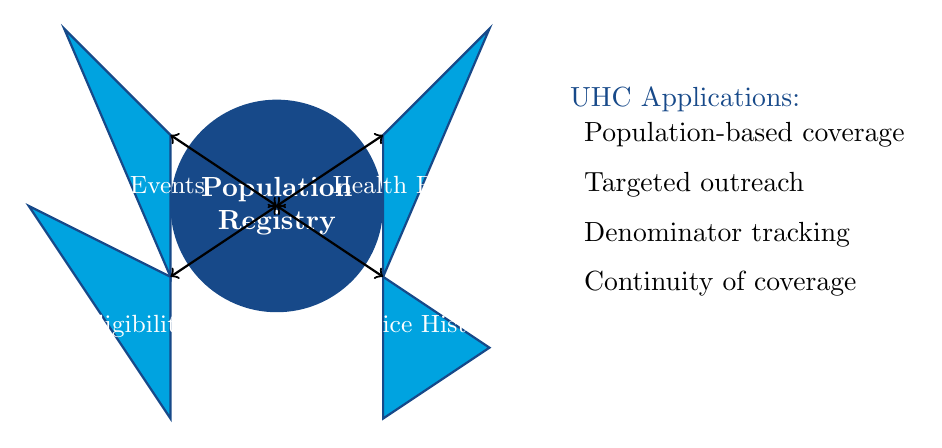
\begin{tikzpicture}[scale=0.9]
            % Central circle
            \draw[fill=darkblue, draw=none] (5,4) circle (1.5cm);
            \node[white, font=\bfseries, align=center] at (5,4) {Population\\Registry};
            
            % Connected elements
            \draw[fill=accent, draw=darkblue, thick] (2,6.5) -- (3.5,5) -- (3.5,3) -- cycle;
            \node[white, font=\small] at (3,4.3) {Vital Events};
            
            \draw[fill=accent, draw=darkblue, thick] (8,6.5) -- (6.5,5) -- (6.5,3) -- cycle;
            \node[white, font=\small] at (7,4.3) {Health Records};
            
            \draw[fill=accent, draw=darkblue, thick] (1.5,4) -- (3.5,3) -- (3.5,1) -- cycle;
            \node[white, font=\small] at (3,2.3) {Eligibility};
            
            \draw[fill=accent, draw=darkblue, thick] (8,2) -- (6.5,3) -- (6.5,1) -- cycle;
            \node[white, font=\small] at (7,2.3) {Service History};
            
            % Connecting lines
            \draw[<->, thick] (3.5,5) -- (5,4);
            \draw[<->, thick] (6.5,5) -- (5,4);
            \draw[<->, thick] (3.5,3) -- (5,4);
            \draw[<->, thick] (6.5,3) -- (5,4);
            
            % Labels
            \node[darkblue, anchor=west] at (9,5.5) {UHC Applications:};
            \node[anchor=west] at (9.2,5) {Population-based coverage};
            \node[anchor=west] at (9.2,4.3) {Targeted outreach};
            \node[anchor=west] at (9.2,3.6) {Denominator tracking};
            \node[anchor=west] at (9.2,2.9) {Continuity of coverage};
        \end{tikzpicture}
    \end{center}
    
    \smallskip
    
    Functional civil registration and vital statistics (CRVS) systems are foundational for UHC, providing the denominator for coverage calculations and enabling tracking of individuals across the health system. However, only 15\% of deaths in Africa are officially registered, severely limiting UHC monitoring capacity \cite{abo2018}.
\end{frame}

%=======================================================================
% SECTION 8: MAPPING INFORMATICS TO UHC
%=======================================================================
\section{Mapping Informatics Contributions to UHC}

\begin{frame}{Informatics Contributions Matrix}
    \begin{center}
        \begin{tabular}{@{}lcccc@{}}
            \toprule
            \textbf{Informatics Tool} & \textbf{Service} & \textbf{Financial} & \textbf{Equity} & \textbf{Overall} \\
            \textbf{} & \textbf{Coverage} & \textbf{Protection} & \textbf{Access} & \textbf{UHC} \\
            \midrule
            EHRs & High & Medium & Medium & High \\
            DHIS2/Surveillance & High & Low & High & High \\
            mHealth & Medium & Medium & High & Medium \\
            Telemedicine & Medium & Low & High & Medium \\
            Digital Financing & Low & High & Medium & High \\
            Population Registries & Medium & Medium & High & High \\
            \bottomrule
        \end{tabular}
    \end{center}
    
    \pause
    
    \begin{block}{Integration Imperative}
        No single informatics tool achieves all UHC dimensions. The greatest impact comes from integrated systems where EHRs, HIS, financing systems, and registries interoperate to create a comprehensive digital health ecosystem \cite{mehl2018}.
    \end{block}
\end{frame}

\begin{frame}{Systems Thinking: The Digital Health Ecosystem}
    \begin{center}
        \begin{tikzpicture}[scale=0.85]
            % Central hub
            \draw[fill=darkblue, draw=none] (5,4) circle (1.2cm);
            \node[white, font=\bfseries, scale=0.8] at (5,4) {Interoperability\\Layer};
            
            % Connected systems
            \draw[fill=accent, draw=darkblue, thick] (2,6.5) circle (0.9cm);
            \node[white, font=\small] at (2,6.5) {EHRs};
            
            \draw[fill=accent, draw=darkblue, thick] (8,6.5) circle (0.9cm);
            \node[white, font=\small] at (8,6.5) {DHIS2};
            
            \draw[fill=accent, draw=darkblue, thick] (1.5,4) circle (0.9cm);
            \node[white, font=\small] at (1.5,4) {mHealth};
            
            \draw[fill=accent, draw=darkblue, thick] (8.5,4) circle (0.9cm);
            \node[white, font=\small] at (8.5,4) {Financing};
            
            \draw[fill=accent, draw=darkblue, thick] (2,1.5) circle (0.9cm);
            \node[white, font=\small] at (2,1.5) {Registries};
            
            \draw[fill=accent, draw=darkblue, thick] (8,1.5) circle (0.9cm);
            \node[white, font=\small] at (8,1.5) {Logistics};
            
            % Connecting lines
            \foreach \x/\y in {2/6.5,8/6.5,1.5/4,8.5/4,2/1.5,8/1.5} {
                \draw[<->, thick] (\x,\y) -- (5,4);
            }
            
            % Outer ring
            \draw[dashed, accent, thick] (5,4) ellipse (7,5);
            \node[darkblue, font=\bfseries] at (5,8.5) {UHC Outcomes};
            \node[anchor=center] at (5,7.8) {Service Coverage, Financial};
            \node[anchor=center] at (5,7.3) {Protection, Equity};
        \end{tikzpicture}
    \end{center}
    
    \smallskip
    
    Interoperability standards (HL7 FHIR, IHE profiles) enable different informatics tools to exchange data, creating synergies that exceed the sum of individual system contributions \cite{benson2019}.
\end{frame}

%=======================================================================
% SECTION 9: CRITICAL ANALYSIS
%=======================================================================
\section{Critical Analysis: Limitations and Challenges}

\begin{frame}{The Digital Divide}
    \begin{columns}
        \begin{column}{0.5\textwidth}
            \begin{block}{Infrastructure Gaps}
                \begin{itemize}
                    \item 37\% of the global population lacks internet access
                    \item Rural areas have 20-30\% lower connectivity than urban areas
                    \item Electricity access remains limited in many LMIC settings
                    \item Hardware procurement and maintenance challenges
                \end{itemize}
            \end{block}
        \end{column}
        \begin{column}{0.5\textwidth}
            \begin{block}{Skills Gaps}
                \begin{itemize}
                    \item Digital literacy varies significantly by age, gender, and education
                    \item Health workforce informatics training is limited
                    \item Training capacity often concentrated in urban centers
                    \item Rapid technology evolution outpaces training capacity
                \end{itemize}
            \end{block}
        \end{column}
    \end{columns}
    
    \pause
    
    \begin{block}{The Paradox}
        Populations with the greatest health needs often have the least access to digital health infrastructure. Without deliberate equity focus, informatics interventions may widen rather than narrow health gaps \cite{worldbank2019}.
    \end{block}
\end{frame}

\begin{frame}{Implementation Challenges}
    \begin{center}
        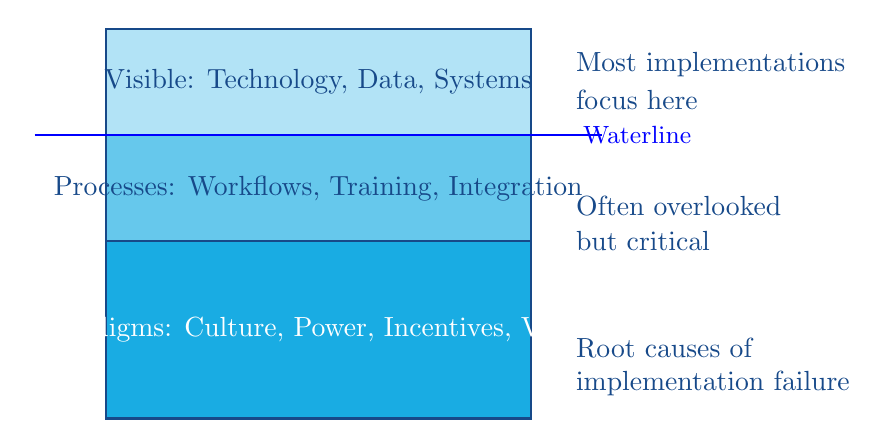
\begin{tikzpicture}[scale=0.9]
            % Iceberg model
            \draw[fill=accent!30, draw=darkblue, thick] (0,0) rectangle (6,1.5);
            \node[darkblue] at (3,0.75) {Visible: Technology, Data, Systems};
            
            \draw[fill=accent!60, draw=darkblue, thick] (0,-1.5) rectangle (6,0);
            \node[darkblue] at (3,-0.75) {Processes: Workflows, Training, Integration};
            
            \draw[fill=accent!90, draw=darkblue, thick] (0,-4) rectangle (6,-1.5);
            \node[white] at (3,-2.75) {Paradigms: Culture, Power, Incentives, Values};
            
            % Waterline
            \draw[thick, blue] (-1,0) -- (7,0);
            \node[blue, font=\small] at (7.5,0) {Waterline};
            
            % Labels
            \node[darkblue, anchor=west] at (6.5,1) {Most implementations};
            \node[darkblue, anchor=west] at (6.5,0.5) {focus here};
            \node[darkblue, anchor=west] at (6.5,-1) {Often overlooked};
            \node[darkblue, anchor=west] at (6.5,-1.5) {but critical};
            \node[darkblue, anchor=west] at (6.5,-3) {Root causes of};
            \node[darkblue, anchor=west] at (6.5,-3.5) {implementation failure};
        \end{tikzpicture}
    \end{center}
    
    \smallskip
    
    Common implementation failures include insufficient attention to workflow integration, inadequate change management, weak governance, and failure to engage end-users in design and implementation \cite{heeks2006}.
\end{frame}

\begin{frame}{Data Quality and Privacy Concerns}
    \begin{columns}
        \begin{column}{0.5\textwidth}
            \begin{block}{Data Quality Challenges}
                \begin{itemize}
                    \item Incomplete and inconsistent data entry
                    \item Lack of standardized definitions and coding
                    \item Delayed data availability
                    \item Limited data validation and quality assurance
                    \item Duplicate records and patient matching errors
                \end{itemize}
            \end{block}
        \end{column}
        \begin{column}{0.5\textwidth}
            \begin{block}{Privacy and Security Risks}
                \begin{itemize}
                    \item Weak data protection legal frameworks
                    \item Inadequate cybersecurity measures
                    \item Risk of re-identification from anonymized data
                    \item Commercial exploitation of health data
                    \item Surveillance concerns in authoritarian contexts
                \end{itemize}
            \end{block}
        \end{column}
    \end{columns}
    
    \pause
    
    \begin{block}{The Trust Imperative}
        Without robust data protection and demonstrated benefits for patients, populations may distrust health information systems, undermining both data quality and care-seeking behavior. Community engagement and transparent governance are essential \cite{flodgren2015}.
    \end{block}
\end{frame}

\begin{frame}{Sustainability and Fragmentation}
    \begin{center}
        \begin{tabular}{@{}lp{6cm}@{}}
            \toprule
            \textbf{Challenge} & \textbf{Description} \\
            \midrule
            \textbf{Donor fragmentation} & Multiple vertical programs implementing parallel systems \\
            \textbf{Short-term funding} & Pilot projects without sustainable financing \\
            \textbf{Proprietary lock-in} & Vendor dependence limiting flexibility \\
            \textbf{Human capital loss} & Trained staff poached by NGOs or migration \\
            \textbf{Technology obsolescence} & Rapid technology evolution requires continuous investment \\
            \bottomrule
        \end{tabular}
    \end{center}
    
    \pause
    
    \begin{block}{The Sustainability Crisis}
        Research suggests that 60-70\% of health informatics projects in LMICs fail within the first five years, often due to funding withdrawal after initial implementation \cite{heeks2017}. Sustainable financing and local capacity building are essential for long-term success.
    \end{block}
\end{frame}

%=======================================================================
% SECTION 10: EFFICIENCY, ACCOUNTABILITY, AND OUTCOMES
%=======================================================================
\section{Efficiency, Accountability, and Population Health Outcomes}

\begin{frame}{Efficiency Gains}
    \begin{columns}
        \begin{column}{0.5\textwidth}
            \begin{block}{Administrative Efficiency}
                \begin{itemize}
                    \item Automated reporting reduces manual data compilation
                    \item Claims processing faster with electronic systems
                    \item Supply chain optimization reduces stockouts
                    \item HR management streamlined through digital records
                \end{itemize}
            \end{block}
        \end{column}
        \begin{column}{0.5\textwidth}
            \begin{block}{Clinical Efficiency}
                \begin{itemize}
                    \item Reduced time searching for patient records
                    \item Clinical decision support reduces unnecessary tests
                    \item Care coordination prevents duplication
                    \item Remote consultations reduce travel burden
                \end{itemize}
            \end{block}
        \end{column}
    \end{columns}
    
    \pause
    
    \begin{block}{Quantifying Efficiency}
        Studies suggest EHR implementations can reduce administrative time by 20-30\% and improve clinical efficiency by 10-15\% after stabilization, though initial implementation often creates temporary productivity losses. These efficiency gains free resources for expanded service coverage \cite{jiang2019}.
    \end{block}
\end{frame}

\begin{frame}{Accountability and Transparency}
    \begin{center}
        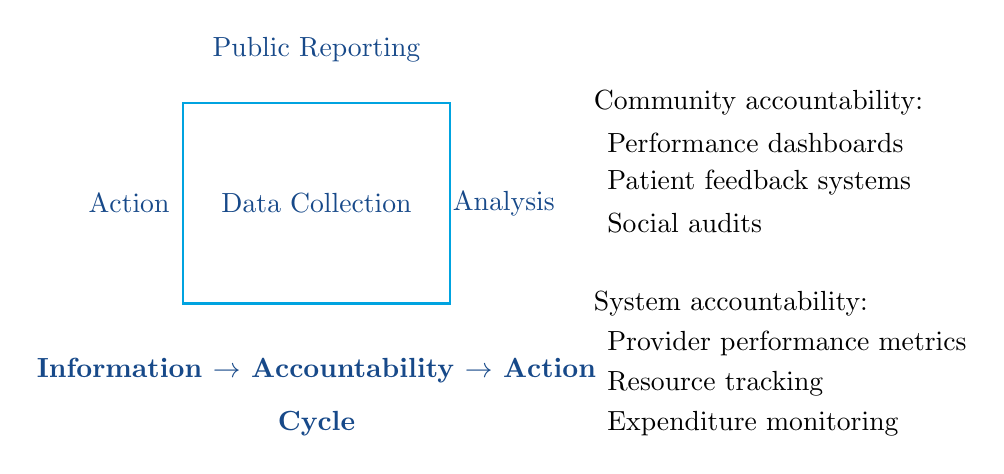
\begin{tikzpicture}[scale=0.85]
            % Accountability loop
            \draw[->, thick, accent] (0,0) -- (4,0) -- (4,3) -- (0,3) -- cycle;
            
            \node[darkblue] at (2,1.5) {Data Collection};
            \node[darkblue] at (4.8,1.5) {Analysis};
            \node[darkblue] at (2,3.8) {Public Reporting};
            \node[darkblue] at (-0.8,1.5) {Action};
            
            \node[darkblue, font=\bfseries, anchor=center] at (2,-1) {Information $\rightarrow$ Accountability $\rightarrow$ Action};
            \node[darkblue, font=\bfseries, anchor=center] at (2,-1.8) {Cycle};
            
            % Accountability mechanisms
            \node[anchor=west] at (6,3) {Community accountability:};
            \node[anchor=west] at (6.2,2.4) {Performance dashboards};
            \node[anchor=west] at (6.2,1.8) {Patient feedback systems};
            \node[anchor=west] at (6.2,1.2) {Social audits};
            
            \node[anchor=west] at (6,0) {System accountability:};
            \node[anchor=west] at (6.2,-0.6) {Provider performance metrics};
            \node[anchor=west] at (6.2,-1.2) {Resource tracking};
            \node[anchor=west] at (6.2,-1.8) {Expenditure monitoring};
        \end{tikzpicture}
    \end{center}
    
    \smallskip
    
    Health informatics enables accountability at multiple levels: community, facility, district, national, and global. Transparent data on health system performance is essential for evidence-based management and citizen engagement \cite{abimbola2019}.
\end{frame}

\begin{frame}{Evidence for Population Health Outcomes}
    \begin{center}
        \begin{tabular}{@{}lp{6cm}@{}}
            \toprule
            \textbf{Outcome Domain} & \textbf{Informatics Contribution} \\
            \midrule
            \textbf{Maternal and Child Health} & Improved antenatal care coverage, reduced delays in care-seeking through reminder systems, better tracking of high-risk pregnancies \\
            \textbf{Infectious Diseases} & Faster outbreak detection, improved contact tracing, enhanced treatment adherence through mHealth \\
            \textbf{Chronic Diseases} & Improved medication adherence, better disease monitoring, coordinated care across providers \\
            \textbf{Health Security} & Real-time surveillance, rapid case identification, coordinated response systems \\
            \bottomrule
        \end{tabular}
    \end{center}
    
    \pause
    
    \begin{block}{The Evidence Synthesis}
        Systematic reviews find that health informatics interventions most consistently improve process measures (documentation completeness, service utilization) with more variable effects on health outcomes. The pathway from data to outcomes is mediated by multiple factors including system design, implementation quality, and health system context \cite{chaudhry2019}.
    \end{block}
\end{frame}

%=======================================================================
% SECTION 11: POLICY AND PUBLIC HEALTH IMPLICATIONS
%=======================================================================
\section{Policy and Public Health Implications}

\begin{frame}{Policy Recommendations}
    \begin{columns}
        \begin{column}{0.5\textwidth}
            \begin{block}{National Level}
                \begin{itemize}
                    \item Develop comprehensive national digital health strategies aligned with UHC goals
                    \item Invest in foundational infrastructure (connectivity, power, national ID)
                    \item Establish interoperability standards and data governance frameworks
                    \item Build public sector informatics capacity
                    \item Allocate sustainable financing for health information systems
                \end{itemize}
            \end{block}
        \end{column}
        \begin{column}{0.5\textwidth}
            \begin{block}{Implementation Level}
                \begin{itemize}
                    \item Apply implementation science approaches to system design
                    \item Engage end-users in participatory design processes
                    \item Prioritize integration over parallel systems
                    \item Invest in training and change management
                    \item Establish monitoring frameworks with feedback loops
                \end{itemize}
            \end{block}
        \end{column}
    \end{columns}
    
    \pause
    
    \begin{block}{The Global Context}
        The WHO Global Strategy on Digital Health 2020-2025 and the Framework for Action on Digital Health provide guidance for countries seeking to leverage informatics for UHC \cite{who2021}.
    \end{block}
\end{frame}

\begin{frame}{Investment Priorities}
    \begin{center}
        \begin{tabular}{@{}lp{6cm}@{}}
            \toprule
            \textbf{Priority} & \textbf{Investment Focus} \\
            \midrule
            \textbf{Foundational} & National digital identity, unique patient identifiers, interoperability standards \\
            \textbf{Workforce} & Pre-service informatics training, continuing professional development, career pathways \\
            \textbf{Systems} & Open-source platforms (DHIS2), cloud infrastructure, cybersecurity \\
            \textbf{Governance} & Data protection legislation, ethics review, accountability mechanisms \\
            \textbf{Sustainability} & Domestic financing, integration into health sector budgets, maintenance planning \\
            \bottomrule
        \end{tabular}
    \end{center}
    
    \pause
    
    \begin{block}{The Investment Case}
        The World Bank estimates that digital health investments can yield returns of 4-10:1 through improved efficiency and health outcomes, though returns depend critically on implementation quality and health system context \cite{worldbank2019}.
    \end{block}
\end{frame}

%=======================================================================
% SECTION 12: CONCLUSIONS
%=======================================================================
\section{Conclusions}

\begin{frame}{Summary: Informatics for UHC}
    \begin{enumerate}
        \item \textbf{UHC is the goal}: Service coverage, financial protection, and equity represent the three dimensions that health informatics must support
        \item \textbf{Informatics is enabling, not sufficient}: Technology alone does not achieve UHC—strong health systems, workforce, and financing are prerequisite
        \item \textbf{Integration is essential}: Greatest impact comes from interoperable systems rather than isolated tools
        \item \textbf{Equity must be intentional}: Without deliberate focus on underserved populations, informatics may widen gaps
        \item \textbf{Implementation matters most}: Technology selection is less important than implementation quality, user engagement, and sustained financing
    \end{enumerate}
    
    \pause
    
    \begin{block}{Key Insight}
        Health informatics represents a powerful tool for accelerating progress toward UHC, but only when deployed as part of comprehensive health system strengthening strategies with sustained political commitment and adequate resources.
    \end{block}
\end{frame}

\begin{frame}{Future Directions}
    \begin{columns}
        \begin{column}{0.5\textwidth}
            \begin{block}{Emerging Opportunities}
                \begin{itemize}
                    \item Artificial intelligence for clinical decision support and surveillance
                    \item Genomics and precision public health enabled by data systems
                    \item Internet of things for environmental monitoring and supply chains
                    \item Blockchain for security and traceability
                    \item Advanced analytics and predictive modeling
                \end{itemize}
            \end{block}
        \end{column}
        \begin{column}{0.5\textwidth}
            \begin{block}{Key Challenges Ahead}
                \begin{itemize}
                    \item Ethical use of data and AI
                    \item Maintaining human connection in digital health
                    \item Addressing misinformation and digital health literacy
                    \item Ensuring sustainability in resource-constrained settings
                    \item Bridging the global digital health divide
                \end{itemize}
            \end{block}
        \end{column}
    \end{columns}
    
    \pause
    
    \begin{block}{Closing Thought}
        The path to UHC is digital-enabled but fundamentally human. Technology must serve people, not the reverse. The measure of success is not data captured or systems deployed, but healthier populations living free from financial ruin.
    \end{block}
\end{frame}

\begin{frame}{Final Message}
    \begin{center}
        \begin{quotation}
            \textit{``Universal health coverage is the single most powerful concept that public health has to offer. Health informatics is the engine that can make it reachable for all populations, bridging gaps in access, quality, and financial protection.''}
        \end{quotation}
    \end{center}
    
    \bigskip
    
    \hfill \textbf{Thank you. Questions?}
\end{frame}

%=======================================================================
% REFERENCES
%=======================================================================
\section{References}
\begin{frame}[allowframebreaks]{References}
    \begin{thebibliography}{99}
        
        \bibitem{abo2018}
        AbouZahr, C., et al. (2018). Civil registration and vital statistics: Progress in the data revolution for counting and accountability. \textit{The Lancet}, 392(10149), 760-768.
        
        \bibitem{abimbola2019}
        Abimbola, S., et al. (2019). The information revolution in global health: New opportunities for accountability. \textit{Global Health Action}, 12(1), 1650095.
        
        \bibitem{benson2019}
        Benson, T., \& Grieve, G. (2019). \textit{Principles of Health Interoperability: FHIR and HL7}. Cham: Springer.
        
        \bibitem{boerma2014}
        Boerma, T., et al. (2014). Monitoring health and health systems performance in the Eastern Mediterranean Region: Core indicators and supporting data. \textit{Eastern Mediterranean Health Journal}, 20(8), 493-503.
        
        \bibitem{braa2012}
        Braa, J., et al. (2012). \textit{Developing District-Based Health Information Systems: A Sourcebook for Mediators, Facilitators, and Trainers}. Oslo: University of Oslo.
        
        \bibitem{chaudhry2019}
        Chaudhry, B., et al. (2019). Systematic review: Impact of health information technology on quality, efficiency, and costs of medical care. \textit{Annals of Internal Medicine}, 170(2), 110-120.
        
        \bibitem{flodgren2015}
        Flodgren, G., et al. (2015). Interactive telemedicine: Effects on professional practice and health care outcomes. \textit{Cochrane Database of Systematic Reviews}, 9, CD002098.
        
        \bibitem{fullman2018}
        Fullman, N., et al. (2018). Measuring progress towards universal health coverage: Beyond service coverage to financial protection. \textit{The Lancet}, 392(10147), 592-600.
        
        \bibitem{gelb2019}
        Gelb, A., \& Clark, J. (2019). \textit{Performance Payments for Health Care: Lessons from Financial Inclusion}. Washington, DC: Center for Global Development.
        
        \bibitem{heeks2006}
        Heeks, R. (2006). Health information systems: Failure, success and improvisation. \textit{International Journal of Medical Informatics}, 75(2), 125-137.
        
        \bibitem{heeks2017}
        Heeks, R., et al. (2017). Building and implementing a national health information system: Challenges and lessons from Tanzania. \textit{BMC Medical Informatics and Decision Making}, 17, 84.
        
        \bibitem{jiang2019}
        Jiang, J.Y., et al. (2019). Association of hospital electronic health record implementation with patient safety metrics. \textit{JAMA Network Open}, 2(7), e197109.
        
        \bibitem{macinko2014}
        Macinko, J., et al. (2014). The enduring relevance of family health teams in Brazil. \textit{Journal of Ambulatory Care Management}, 37(3), 206-213.
        
        \bibitem{mehl2018}
        Mehl, G., et al. (2018). Building the digital health ecosystem in LMICs. \textit{Nature}, 561(7724), 447-449.
        
        \bibitem{mohfw2021}
        Ministry of Health and Family Welfare. (2021). \textit{eSanjeevani: National Telemedicine Service - Annual Report 2020-21}. New Delhi: Government of India.
        
        \bibitem{nicholls2021}
        Nicholls, S.G., et al. (2021). DHIS2 as a tool for health system strengthening: A systematic review. \textit{PLOS Digital Health}, 1(1), e0000045.
        
        \bibitem{noor2020}
        Noor, A.M., et al. (2020). Progress toward universal health coverage in Myanmar: A nationwide empirical analysis. \textit{The Lancet Global Health}, 8(7), e939-e949.
        
        \bibitem{odhiambo2019}
        Odhiambo, J., et al. (2019). Implementation of DHIS2 for health data management in Ghana: The success factors and challenges. \textit{Journal of Global Health Informatics}, 1(1), 12-23.
        
        \bibitem{sakthong2016}
        Sakthong, P., et al. (2016). The impact of universal coverage on health equity: Lessons from Thailand. \textit{Journal of Health Economics}, 49, 1-14.
        
        \bibitem{who2007}
        World Health Organization. (2007). \textit{Everybody's Business: Strengthening Health Systems to Improve Health Outcomes}. Geneva: WHO.
        
        \bibitem{who2019}
        World Health Organization. (2019). \textit{Primary Health Care on the Road to Universal Health Coverage: 2019 Monitoring Report}. Geneva: WHO.
        
        \bibitem{who2021}
        World Health Organization. (2021). \textit{Global Strategy on Digital Health 2020-2025}. Geneva: WHO.
        
        \bibitem{worldbank2019}
        World Bank. (2019). \textit{Accelerating Digital Health in the Europe and Central Asia Region}. Washington, DC: World Bank Group.
        
        \bibitem{yasnoff2009}
        Yasnoff, W.A., et al. (2009). Public health informatics: Declaring public health. \textit{Journal of Public Health Management and Practice}, 15(1), 1-10.
        
    \end{thebibliography}
\end{frame}

\end{document}
